\documentclass[conference]{IEEEtran}
\IEEEoverridecommandlockouts
% The preceding line is only needed to identify funding in the first footnote. If that is unneeded, please comment it out.
% \usepackage{cite}
\usepackage{amsmath,amssymb,amsfonts}
%\usepackage{algorithmic}
\usepackage[ruled,vlined,lined,linesnumbered,spanish]{algorithm2e}
\usepackage{caption}
\usepackage{graphicx}
\usepackage{hyperref}
\usepackage{multirow}
\usepackage{textcomp}
\usepackage{xcolor}
\usepackage[spanish]{babel}

\hypersetup{colorlinks,linkcolor={blue},citecolor={blue},urlcolor={blue}}

\def\BibTeX{{\rm B\kern-.05em{\sc i\kern-.025em b}\kern-.08em
    T\kern-.1667em\lower.7ex\hbox{E}\kern-.125emX}}
\begin{document}

\title{Paper Title*\\
{\footnotesize \textsuperscript{*}Note: Sub-titles are not captured in Xplore and
should not be used}
\thanks{Identify applicable funding agency here. If none, delete this.}
}

\author{\IEEEauthorblockN{1\textsuperscript{st} Given Name Surname}
\IEEEauthorblockA{\textit{dept. name of organization (of Aff.)} \\
\textit{name of organization (of Aff.)}\\
City, Country \\
email address}
\and
\IEEEauthorblockN{2\textsuperscript{nd} Given Name Surname}
\IEEEauthorblockA{\textit{dept. name of organization (of Aff.)} \\
\textit{name of organization (of Aff.)}\\
City, Country \\
email address}
\and
\IEEEauthorblockN{3\textsuperscript{rd} Given Name Surname}
\IEEEauthorblockA{\textit{dept. name of organization (of Aff.)} \\
\textit{name of organization (of Aff.)}\\
City, Country \\
email address}
\and
\IEEEauthorblockN{4\textsuperscript{th} Given Name Surname}
\IEEEauthorblockA{\textit{dept. name of organization (of Aff.)} \\
\textit{name of organization (of Aff.)}\\
City, Country \\
email address}
\and
\IEEEauthorblockN{5\textsuperscript{th} Given Name Surname}
\IEEEauthorblockA{\textit{dept. name of organization (of Aff.)} \\
\textit{name of organization (of Aff.)}\\
City, Country \\
email address}
\and
\IEEEauthorblockN{6\textsuperscript{th} Given Name Surname}
\IEEEauthorblockA{\textit{dept. name of organization (of Aff.)} \\
\textit{name of organization (of Aff.)}\\
City, Country \\
email address}
}

\maketitle

\begin{abstract}
	Lorem ipsum dolor sit amet, consectetur adipiscing elit. Suspendisse eu interdum est. Sed finibus lacinia sapien, nec molestie metus imperdiet ut. Donec vel malesuada nulla. Fusce sodales metus tellus, sit amet mattis risus commodo eget. Pellentesque vitae volutpat nulla, efficitur volutpat mauris. Etiam at libero vitae metus finibus accumsan. Nunc luctus vehicula leo nec dictum. Nullam eget mollis mauris. Etiam ex justo, auctor a arcu eu, elementum convallis lectus. Pellentesque quis lacus et erat lobortis lacinia. Fusce suscipit sem sit amet maximus porttitor. Phasellus consectetur tempus vehicula. Donec dapibus metus vitae magna sodales suscipit. Quisque dignissim massa id suscipit vehicula. 
\end{abstract}

\begin{IEEEkeywords}
	component, formatting, style, styling, insert
\end{IEEEkeywords}

\section{Introduction}
	Proin mollis feugiat lacus sit amet egestas. Aliquam non augue iaculis, semper urna sed, suscipit orci. Nulla sem mi, efficitur et magna a, fringilla suscipit lorem. Sed eget cursus elit, at pretium augue. Ut aliquam vel dui et iaculis. Fusce tempor ipsum in purus tincidunt vulputate. Nam ac purus orci. Etiam maximus porttitor sollicitudin. Maecenas magna leo, pulvinar eget suscipit et, efficitur eget nisl. Maecenas sagittis tempus consectetur. Duis et eros sit amet augue venenatis viverra. Duis non rutrum lacus.

\section{Background}
	\subsection{Was ist Lorem Ipsum}
		Lorem Ipsum ist ein einfacher Demo-Text für die Print- und Schriftindustrie. Lorem Ipsum ist in der Industrie bereits der Standard Demo-Text seit 1500, als ein unbekannter Schriftsteller eine Hand voll Wörter nahm und diese durcheinander warf um ein Musterbuch zu erstellen.

	\subsection{Warum nutzen wir es}
		Es ist ein lang erwiesener Fakt, dass ein Leser vom Text abgelenkt wird, wenn er sich ein Layout ansieht. Der Punkt, Lorem Ipsum zu nutzen, ist, dass es mehr oder weniger die normale Anordnung von Buchstaben darstellt und somit nach lesbarer Sprache aussieht. Viele Desktop Publisher und Webeditoren nutzen mittlerweile Lorem Ipsum

\section{Proposal}
	Before you begin to format your paper, first write and save the content as a 
	separate text file. Complete all content and organizational editing before 
	formatting. Please note sections \ref{AA}--\ref{SCM} below for more information on 
	proofreading, spelling and grammar.

	\subsection{Abbreviations and Acronyms}\label{AA}
		Define abbreviations and acronyms the first time they are used in the text, 
		even after they have been defined in the abstract. Abbreviations such as 
		IEEE, SI, MKS, CGS, ac, dc, and rms do not have to be defined. Do not use 
		abbreviations in the title or heads unless they are unavoidable.

	\subsection{Units}
		\begin{itemize}
			\item Use either SI (MKS) or CGS as primary units. (SI units are encouraged.) English units may be used as secondary units (in parentheses). An exception would be the use of English units as identifiers in trade, such as ``3.5-inch disk drive''.
			\item Avoid combining SI and CGS units, such as current in amperes and magnetic field in oersteds. This often leads to confusion because equations do not balance dimensionally. If you must use mixed units, clearly state the units for each quantity that you use in an equation.
			\item Do not mix complete spellings and abbreviations of units: ``Wb/m\textsuperscript{2}'' or ``webers per square meter'', not ``webers/m\textsuperscript{2}''. Spell out units when they appear in text: ``. . . a few henries'', not ``. . . a few H''.
			\item Use a zero before decimal points: ``0.25'', not ``.25''. Use ``cm\textsuperscript{3}'', not ``cc''.)
		\end{itemize}

	\subsection{Equations}
		Number equations consecutively. To make your 
		equations more compact, you may use the solidus (~/~), the exp function, or 
		appropriate exponents. Italicize Roman symbols for quantities and variables, 
		but not Greek symbols. Use a long dash rather than a hyphen for a minus 
		sign. Punctuate equations with commas or periods when they are part of a 
		sentence, as in:
		\begin{equation}
			a+b=\gamma
			\label{eq:sum}
		\end{equation}

		Be sure that the 
		symbols in your equation have been defined before or immediately following 
		the equation. Use equation ``\ref{eq:sum}''.

	\subsection{Algorithms}\label{SCM}
		\textbf{The class file is designed for, but not limited to, six authors.}.
		Please note that the \verb|{subequations}| environment in {\LaTeX}
		will increment the main equation counter even when there are no
		equation numbers displayed. If you forget that, you might write an
		article in which the equation numbers skip from (17) to (20), causing
		the copy editors to wonder if you've discovered a new method of
		counting. \\
		An excellent style manual for science writers is \cite{cuevas2013} and algorithm \ref{algo:fisrt}.
		
		\begin{algorithm}
			\SetAlgoLined
			\KwIn{Your Input}
			\KwOut{Your output}
			\KwData{Testing set $x$}
			\KwResult{Write here the result }

			initialization\;
			\While{While condition}{
			instructions\;
			\eIf{condition}{
			instructions1\;
			instructions2\;
			}{
			instructions3\;
			}
			}
			\caption{How to write algorithms}
			\label{algo:fisrt}
		\end{algorithm}

\section{Experiment}
	\subsection{Figures and Tables}
		\paragraph{Positioning Figures and Tables} Place figures and tables at the top and 
		bottom of columns. Avoid placing them in the middle of columns. Large 
		figures and tables may span across both columns. Figure captions should be 
		below the figures; table heads should appear above the tables. Insert 
		figures and tables after they are cited in the text. Use the abbreviation 
		``Fig.~\ref{fig:communication}'', even at the beginning of a sentence and table \ref{tab:tgrade}.

		\begin{table}[htbp]
			\caption{Title}
			\begin{center}
			\begin{tabular}{|c|c|c|}
				\hline
				\textbf{Topología}      & \textbf{N° de nodos} & \textbf{Grado} \\ \hline
				Anillo                               & 24                   & 1              \\ \hline
				\multirow{3}{*}{Árbol} & 8                    & 1              \\ \cline{2-3} 
														& 20                   & 2              \\ \cline{2-3} 
														& 6                    & 3              \\ \hline
				\multirow{2}{*}{Red A} & 16                   & 3              \\ \cline{2-3} 
														& 8                    & 4              \\ \hline
				\multirow{2}{*}{Red B} & 20                   & 3              \\ \cline{2-3} 
														& 4                    & 4              \\ \hline
				Toroide                        & 24                   & 4              \\ \hline
				Grafo                            & 24                   & 23             \\ \hline
				\end{tabular}
			\label{tab:tgrade}
			\end{center}
		\end{table}
        
		\begin{figure}[htb]
			\centering
			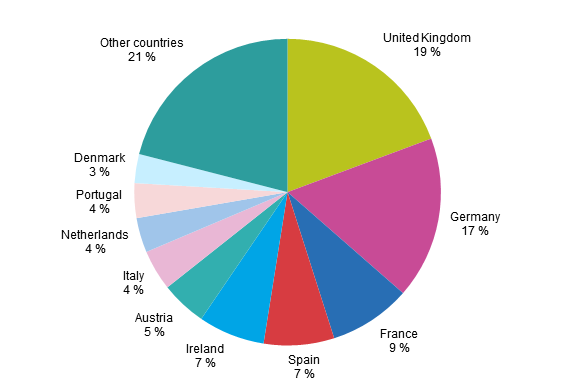
\includegraphics[scale=0.6]{img/fig1.png}
			\caption{Title}
			\captionsetup{font={footnotesize,bf,it}}
			\caption*{Fuente: \cite{cuevas2013}}
			\label{fig:communication}
		\end{figure}

		Figure Labels: Use 8 point Times New Roman for Figure labels. Use words 
		rather than symbols or abbreviations when writing Figure axis labels to 
		avoid confusing the reader. As an example, write the quantity 
		``Magnetization'', or ``Magnetization, M'', not just ``M''. If including 
		units in the label, present them within parentheses. Do not label axes only 
		with units. In the example, write ``Magnetization (A/m)'' or ``Magnetization 
		\{A[m(1)]\}'', not just ``A/m''. Do not label axes with a ratio of 
		quantities and units. For example, write ``Temperature (K)'', not 
		``Temperature/K''.

\section{Result and discussion}
	Es gibt viele Variationen der Passages des Lorem Ipsum, aber der Hauptteil erlitt Änderungen in irgendeiner Form, durch Humor oder zufällige Wörter welche nicht einmal ansatzweise glaubwürdig aussehen. Wenn du eine Passage des Lorem Ipsum nutzt, solltest du aufpassen dass in der Mitte des Textes keine ungewollten Wörter stehen. Viele der Generatoren im Internet neigen dazu, vorgefertigte Stücke zu wiederholen.

\section{Conclusion}
	Lorem Ipsum ist ein einfacher Demo-Text für die Print- und Schriftindustrie. Lorem Ipsum ist in der Industrie bereits der Standard Demo-Text seit 1500, als ein unbekannter Schriftsteller eine Hand voll Wörter nahm und diese durcheinander warf um ein Musterbuch zu erstellen. Es hat nicht nur 5 Jahrhunderte überlebt, sondern auch in Spruch in die elektronische Schriftbearbeitung geschafft (bemerke, nahezu unverändert). Bekannt wurde es 1960, mit dem erscheinen von "Letraset", welches Passagen von Lorem Ipsum enhielt, so wie Desktop Software wie "Aldus PageMaker" - ebenfalls mit Lorem Ipsum.
	
\bibliography{references} % Path to your References.bib file
\bibliographystyle{apalike}
%\bibliographystyle{plainnat} % use this to have URLs listed in References

\end{document}
